\documentclass[tikz,border=5]{standalone}

\pgfdeclareradialshading[droplet color]{droplet}{\pgfqpoint{-10bp}{-10bp}}{%
 color(0bp)=(droplet color!50!white);
 color(9bp)=(droplet color!75!white);
 color(18bp)=(droplet color!85!black);
 color(25bp)=(droplet color);
 color(50bp)=(droplet color!50!white)}

\colorlet{droplet color}{blue!50!cyan}
\tikzset{%
  raindrop/.pic={
    code={\tikzset{scale=1/10}
 \shade [shading=droplet]
 (0,0)  .. controls ++(0,-1) and ++(0,1) .. (1,-2)
 arc (360:180:1)
 .. controls ++(0,1) and ++(0,-1) .. (0,0) -- cycle;
  }}}

\begin{document}
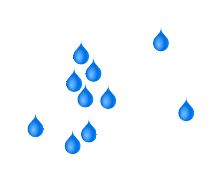
\begin{tikzpicture}
\foreach \i in {1,...,10}
  \path (rand,-\i/8+rand/4) pic {raindrop};
\end{tikzpicture}
\end{document}